\chapter{Methodology} \label{method}

\bigskip \bigskip A systematic approach towards development of a knowledge model can be found in the works of Roy et al. \cite{Roy2004} and Plant et al. \cite{Plant2003}. However, for the purpose of this thesis, developing a knowledge model for industrial risk assessments involves a systematic approach that includes the following steps:
\begin{itemize}
    \item \textbf{Scope and purpose of the knowledge model:} The first step is to identify the specific processes, products, and systems that will be covered by the knowledge model. The purpose of the knowledge model should also be clearly defined, including the type of risk assessment it will support and the stakeholders who will use it. This section of the thesis mainly deals with RQ 1 and evaluates Hypothesis 1.1.
    \item \textbf{Gather relevant data:} The next step is to gather relevant data from various sources. Knowledge from safety standards and knowledge from experts are the main source of knowledge for this work. The data should be organized in a structured format that can be easily searched and analyzed. 
    \item \textbf{Define the knowledge model:} The knowledge model should be designed to capture the relevant information from safety standards, products covered and knowledge from experts. This includes defining the entities, attributes, and relationships that are important for risk assessment.
    \item \textbf{Develop the knowledge model:} Once the knowledge model has been defined, it can be developed using a variety of methods and tools to support the chosen method. Different methods to model knowledge are defined in Section \ref{how_to_model}. This part mainly deals with RQ 2 and evaluates Hypothesis 2. 
    \item \textbf{Implement the knowledge model:} The knowledge model should be integrated into the current risk assessment process. By doing this it becomes easier to validate the model and its output. This involves working for RQ 3 and evaluate Hypothesis 3.1.
    \item \textbf{Validate the knowledge model:} The knowledge model should be validated to ensure its accuracy and reliability. This section of the thesis mainly deals with RQ 4 and evaluates Hypothesis 4.
    \item \textbf{Maintain and update the knowledge model:} It should be possible to regularly review and update the knowledge model to ensure that it remains current and relevant. This may involve incorporating new data or knowledge, refining the model based on feedback from users, or updating it to reflect changes in safety standards or regulations. Also for future applications it should be easy to grow the model with newer safety standards and risk assessments.
\end{itemize}

The implementation and validation of the knowledge model are not really a part of the methodology to build the knowledge model. These topics would come after the model is built, so they are considered as separate chapters after methodology. Also, maintenance and updating the knowledge model is discussed in between other topics. So, it is not separately discussed.

\paragraph{} Developing a knowledge model for industrial risk assessments requires a multidisciplinary approach that involves dealing with data from risk assessments, semantic data from safety standard and exploring the field of Natural Language Processing to reduce manual effort in the process. Also developing the knowledge graph from scratch involves the idea of ontology and semantic triples which are explained further in this chapter.

\section{Scope and purpose of the knowledge model} \label{scope}

\subsection{Scope of the model}
For this project, Hypothesis 1.1 proposed can be considered effective and Hypothesis 1.2 can be nullified as it is a customer-centric approach. Hypothesis 1.2 considers developing the knowledge model from engineering files of each customer which is specific to machine type. This approach may focus too heavily on meeting the customer's needs and expectations, for the particular machine used potentially overlooking important safety considerations. This can lead to a higher risk of accidents that could have been prevented. Also this approach rejects the idea of reusing previous risk assessments which does not make it a fast and efficient approach for future risk assessments. On the other hand, Hypothesis 1.1 is a project-centric approach and can be applicable for machinery of multiple customers. This approach is based on safety standards which are generalized. The following arguments can be made in favour of Hypothesis 1.1:
\begin{enumerate}
    \item Safety standards are based on industry-wide best practices and regulatory requirements, which means they are developed by experts and have been proven effective in promoting safety and reducing risk. 
    \item A safety standard-centric approach is more comprehensive and covers a wider range of potential risks and hazards. It takes into account not only the customer's needs and expectations, but also the broader context in which the product or service is being used.
    \item Safety standards are legally binding, which means that organizations are required to comply with them. By using a safety standard-centric approach, organizations can ensure that they are meeting their legal obligations and reducing the risk of liability.
    \item Safety standards are regularly reviewed and updated, which means that a safety standard-centric approach can help organizations stay up-to-date with the latest best practices, new hazards and requirements. This is in contrast to the engineering files approach of Hypothesis 1.2, as these data stays constant for the given machine, even if new hazards for the machine type are found later.
    \item Expert knowledge can bring a broader perspective to risk assessment, incorporating information from previous assessments can make the future assessments faster. The expert's interpretation of the standard can help to identify potential hazards and develop more effective mitigation strategies which can be transferred to the knowledge model to make it more effective to use.
\end{enumerate}

So, the knowledge model for faster and efficient industrial risk assessment can be made by digitizing knowledge from domain experts and safety standards. This establishes the ground on which the knowledge model is built.

\subsection{Purpose of the model}
The risk assessment of a laser cutting machine is considered for this thesis. A Type A standard, the EN ISO 12100:2010 is used. A documentation of a previous assessment on the machine in accordance with EN ISO 12100:2010 is used as an expert's knowledge, that can be elicited for developing the knowledge model.

\paragraph{} The purpose of a knowledge model built using knowledge from domain experts and safety standards would be to improve safety and reduce risk. Also to make industrial risk assessments faster and efficient. The model would incorporate relevant safety standards and guidelines, as well as the results of previous risk assessments and expert's interpretation, to provide a comprehensive understanding of potential hazards, preventive measures, location of hazards, risk measure, reason of occurrence, mitigation strategies and other important information that is segregated for each hazard. Now this becomes easier for the engineer to look for the hazard applicable for the machine, search for the preventive measures from the knowledge model and mitigate them easily. This approach is faster and efficient than going through the huge safety standard documents and then interpreting the standard to assess the machine. The model should also be future-ready for applications like machine-to-machine communication as discussed further later in this thesis \ref{m2m}.

\section{Gather relevant data}
\label{gather_relevant_data}

There are two main source of data which are considered for the knowledge model,
\begin{itemize}
    \item Knowledge from safety standard
    \item Knowledge from expert
\end{itemize}

\subsection{Knowledge from safety standard}
Safety standards are usually lengthy and complex documents, and extracting knowledge manually can be a tedious task. However, there are several techniques available in computer science that can be used to automate the process of extracting knowledge from safety standards. Here are some of the techniques that can be used:
\begin{itemize}
    \item \textbf{Natural Language Processing (NLP):} NLP is a technique used to extract information from natural language texts such as safety standards. NLP algorithms can be used to automatically identify the key concepts and relations between concepts, from the safety standards. The concepts and relations can then be used to create structured data that can be easily analyzed.
    \item \textbf{Machine Learning (ML):} ML algorithms can be trained on safety standards to identify patterns and extract information automatically. For example, ML algorithms can be used to identify safety hazards and controls, and categorize them according to their severity.
    \item \textbf{Data Mining:} Data mining techniques can be used to extract information from large datasets of safety standards. These techniques can help identify patterns and relationships in the data, which can be used to develop a comprehensive knowledge model.
\end{itemize}

The machine learning approach and data mining approach are data-intensive. It means that these two techniques need a huge quantity of data to train and test the model. These approaches are useful when there is a large amount of structured data available, such as safety concepts and the relations between the concepts. However, in this project, the only available data source is the EN ISO 12100 safety standard which contains unstructured textual data that is not machine readable. The idea here is to develop such a structured data source that can be used in future by machine learning applications.

\paragraph{} On the other hand, natural language processing (NLP) techniques can be useful when there is limited data available, which is unstructured. NLP techniques can help to identify key concepts and relations from safety standard based on the language used in the document. However, it's important to note that each approach has its own strengths and limitations. For example, ML and data mining approaches may be able to identify complex patterns and relationships in the data that are not easily recognizable through NLP techniques. Similarly, NLP techniques may not be able to identify and connect all safety hazards and controls, concepts and relations that are present in the safety standard.

\paragraph{} Therefore, the best way to go is semi-automatic, which is followed in this work. An NLP algorithm can be helpful to automate the process of information extraction from safety standards, but the process is still heavily dependent on manual effort. This is because safety standards are often complex documents that may contain nuanced information that may be difficult for the NLP algorithm to fully capture. Manual work can help ensure that the extracted information is accurate and relevant to the specific context. This can include reviewing and refining the results of NLP techniques to ensure that they accurately reflect the content of the safety standards. A combination of NLP technique and manual work may be the best approach for developing a comprehensive knowledge model for safety standards and this can help ensure that the extracted information is accurate, relevant, and tailored to the specific context.

\subsubsection{Information extraction pipeline}
An information extraction (IE) pipeline is a series of steps or processes designed to extract structured information from unstructured data, such as text documents. From the work of N. Jain et al. \cite{text2kg} and from the projects demonstrated in \cite{analyticsvidhya} and \cite{medium}, the following pipeline is prepared.

% \bigskip 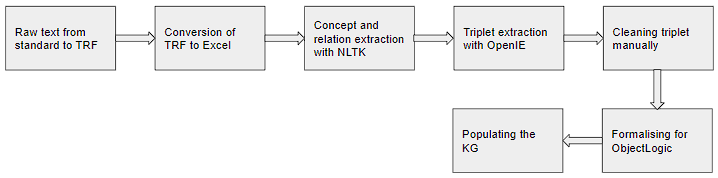
\includegraphics[width=\textwidth]{img/12100_IE_pipeline.png}

\bigskip \adjustimage{width=\textwidth, center, caption={IE pipeline for the safety standard}, label={fig3}, nofloat=figure, vspace=\bigskipamount}{img/12100_IE_pipeline.png}

\paragraph{} The first step is to extract the text from the safety standard which is in .pdf format to a more workable .xlsx format. This is done using a tool which is used to convert a pdf document into a TRF (Test Report Form) and then from the TRF to an excel sheet using a simple Python code. This de-tour for the conversion of the standard from .pdf to .xlsx is used so that the formatting of the original document is preserved. This ensures that the information under each clause as described in the standard is also preserved in the .xlsx format. It ensures that the triplets are created under each clause separately and thus makes the cleaning easier. The TRF or Test Report Form is the document used by experts to perform safety assessment on a machine according to a standard. The excel sheet prepared have the clause numbers on separate column and the requirements on another column. Each requirement per clause is separated by each row. This makes working with the text much easier for the subsequent steps. The effort required is also minimum since the process is automated. 

\paragraph{} Now that the requirements from the standard are extracted in a separate column and each requirement separated into rows, few data cleaning steps must be taken to ensure that the NLP algorithm returns workable results. The information that are not required such as Notes, Examples, Tables, Figures and other data that need not be a part of the final knowledge model can be excluded. This curated column can finally be converted to a pandas dataframe to be an input of the NLP tool used. While researching for this work, there are several tools and libraries found that can assist with various steps in the process of generating a knowledge model from unstructured text, these are:
\begin{itemize}
    \item \textbf{NLTK:} This is a popular Python library for natural language processing, which includes tools for text preprocessing, named entity recognition (NER), and part-of-speech (POS) tagging.
    \item \textbf{Stanford CoreNLP/Stanza:} This is a Java library for NLP that includes tools for tokenization, part-of-speech tagging, dependency parsing, and named entity recognition. A newer version of this package is Stanza which is a Python package and CoreNLP can also be accessed by Stanza via its server interface by launching the Stanford CoreNLP client. 
    \item \textbf{Spacy:} This is another popular Python library for NLP that includes tools for text preprocessing, named entity recognition, part-of-speech tagging, and dependency parsing.
    \item \textbf{OpenIE:} This is a tool for extracting open-domain, subject-predicate-object (SPO) relation triples style information from text, which can be used to construct a knowledge graph. This tool is originally from the Stanford CoreNLP package which can also be accessed via Stanza in a Python environment.
    \item \textbf{ClauseIE:} Clause-based Information Extraction is a type of information extraction technique that focuses on extracting information from specific clauses in text. This tool is the work of Corro et al. \cite{Corro2013}.
\end{itemize}

\subsubsection{Concepts and relation extraction using NLTK}
NLTK (Natural Language Toolkit) provides a variety of tools and methods for extracting concepts and relations from sentences. One approach to extracting concepts and relations from sentences using NLTK involves part-of-speech (POS) tagging. POS tagging is the process of assigning a part-of-speech tag (such as noun, verb, adjective, etc.) to each word in a text document. The goal of POS tagging is to identify the grammatical structure of the text and to disambiguate the meanings of words based on their context. NLTK provides built-in functions for performing POS tagging on texts. Using NLTK, first POS tagging is performed on each sentence to identify the parts of speech of the words in the sentence. Then, rules or patterns are applied to the POS tagged sentence to identify concepts and relations. Here, nouns of all kinds are put to a list as concepts and verbs of all kinds are put to a list as relations. \cite{nltkbook}

\subsubsection{Triple Extraction with OpenIE}
OpenIE (Open Information Extraction) is a technique in natural language processing (NLP) that is used to extract structured information from unstructured or semi-structured text. Unlike traditional named entity recognition (NER) or relation extraction techniques, OpenIE aims to extract relations between entities in a more open-ended and unconstrained way, without relying on pre-defined relation types or hand-labeled training data. OpenIE is often used as a preprocessing step for building knowledge graphs, since it can help automatically identify relationships between entities in large amounts of unstructured text which is demonstrated by the work done by N. Jain et al. \cite{text2kg}. Similar use of OpenIE is done in this work with Stanford CoreNLP OpenIE.

\paragraph{} SPO (Subject-Predicate-Object) triples are a way of representing structured information in a way that can be easily understood and processed by computers. Each SPO triple consists of three components:
\begin{itemize}
    \item \textbf{Subject:} The entity or concept being described
    \item \textbf{Predicate:} The relationship or property between the subject and the object
    \item \textbf{Object:} The entity or value that the subject is related to by the predicate
\end{itemize}
SPO triples are useful for building knowledge models because they provide a way to represent structured information in a machine-readable format. By representing information in terms of SPO triples, a knowledge graph can be built that allows us to make inferences, answer questions, and discover new insights based on the relationships between entities. 

\paragraph{} Since Python is used for this project and Stanford CoreNLP provides OpenIE in the Java environment, a newer Python package from Stanford NLP called Stanza is used. Stanza allows accessing the Java toolkit via its server interface. First the filtered sentences from the dedicated column of the excel sheet is taken as an input and converted to a pandas dataframe to make work easy. Then CoreNLP Server is launched in the background with the annotator as OpenIE sending each sentence from the dataframe to the server one by one. The output for each line is then appended to a dictionary tagging each subject, relation and object separately. For each line there may be more than one triple so the triple dictionaries are appended to a triples list which is the final output for each sentence. This particular structured format of using dictionaries is used so that the process of formalization of the triples to build the final knowledge model could become automatic and simple, which is discussed later in this chapter. Finally each list for each line is written automatically in the working excel. Here, excel is used because of its familiarity and ease of use. The final aim is to prepare the data set to be fed into OntoBroker which is used to prepare the semantic model. Working code for the CoreNLP Client Interface can be cited from the work of P. Qi et al. \cite{stanza}. An example from the safety standard might make the complete process clearer. 
\begin{itemize}
\item Sentence: "Risk analysis provides information required for the risk evaluation, which in turn allows judgments to be made about whether or not risk reduction is required."
\item 'subject': 'Risk analysis', 'relation': 'provides information required for', 'object': 'risk evaluation'
\item 'subject': 'Risk evaluation', 'relation': 'allows judgements to be made', 'object': 'risk reduction'
\end{itemize}

\subsubsection{Manual work}
It is found that the triples generated using OpenIE had a wide variation of SPO combinations for a single sentence. For some sentences the triples generated can be used for building the knowledge model but for some sentences the triples made no sense. Also for some sentences there was no output. The more complex a sentence gets, the more difficult it becomes for the algorithm to give a correct output. This leaves a sweet spot for future research on this topic about how an algorithm can be optimized for automatic generation of SPO triples from unstructured text. However, for the course of this work, manual intervention is required to get the final triples right.

\paragraph{} For sentences where the SPO triples were not extracted correctly, a manual extraction of triples is required. Extracting SPO triples manually from this standard involves reading through the individual sentences and understanding its linkage with neighbouring sentences. Here are some general steps followed:
\begin{itemize}
    \item Read the safety standard: The document is read carefully to understand the context and structure of the content. Most importantly to understand how the clauses are divided and their content.
    \item Identify the relevant information: The information is identified that is relevant to the risk assessment process, such as hazards, risks, preventive measures, and other safety requirements.
    \item Identify the subject: The subject or entity is identified that the information is referring to. This could be a machine, hazard name, process, or other element related to the machinery design.
    \item Identify the predicate: The predicate or relationship between the subject and object is identified. This could be a requirement, recommendation, or other type of relationship.
    \item Identify the object: The object or attribute related to the subject is identified. This could be information on hazard, risk reduction measure, safety requirement information, or other relevant information.
    \item Organize the information into SPO triplets: Once the subject, predicate, and object are identified, the information is organized into SPO triplets in the dictionary format as discussed previously.
\end{itemize}

Here's an example of an SPO triplet that couldn't be extracted automatically, but needs to be extracted manually from the ISO 12100:
\begin{itemize}
    \item Sentence: Electrical hazards - For requirements related to specific machines, see corresponding IEC standards (for example, IEC 61029, IEC 60745 or IEC 60335).
    \item Subject: electrical hazards
    \item Predicate: reference standards
    \item Object: IEC 61029, IEC 60745, IEC 60335
\end{itemize}
    
This information can be organized into an SPO triplet as follows:

[{'subject': 'electrical hazards', 'relation': 'reference standards', 'object': 'IEC 61029'}]

[{'subject': 'electrical hazards', 'relation': 'reference standards', 'object': 'IEC 60745'}]

[{'subject': 'electrical hazards', 'relation': 'reference standards', 'object': 'IEC 60335'}]

\subsection{Knowledge from expert}

% \bigskip 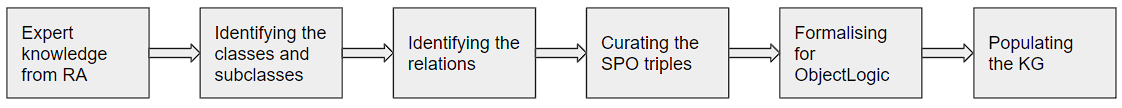
\includegraphics[width=\textwidth]{img/Expert_IE_pipeline.png}

\bigskip \adjustimage{width=\textwidth, center, caption={IE pipeline for the knowledge from expert}, label={fig4}, nofloat=figure, vspace=\bigskipamount}{img/Expert_IE_pipeline.png}

\paragraph{} For this thesis, the risk assessment of a laser cutting machine is considered. The work of Kleen \cite{kleen} is taken as a documentation of previous risk assessment that is done on the laser cutting machine concerned. This machine consists of individual components like robot, laser, transfer station on which risk assessment in accordance with the EN ISO 12100 was performed. These individual reports can be considered to be the knowledge from an expert that is required to build the model. Expert knowledge elicitation from documents involves a process of extracting, categorizing, and organizing information to generate insights and knowledge that can be used to develop the knowledge model. Mostly, the information is in tabular format so unlike the plain textual data from the safety standard, this data is somewhat semi-structured. It is required to understand the structure and identify the pattern that could be used to amalgamate the knowledge from two sources so that the knowledge model could have a homogeneous structure. For example, relations (predicates) are looked for which can match the ones extracted from the safety standard. This matching is done manually to avoid similar meaning triples to be represented differently in the final knowledge model. The data is organized similarly as done for the safety standard, that is, by creating SPO (Subject-Predicate-Object) triples in a dictionary structure. 

\section{Define the knowledge model}\label{class_hierarchy}

After extracting the required data in a structured format, it is required to define a basic outlined structure of the knowledge model. A class hierarchy diagram can be helpful here. A class hierarchy diagram is a visual representation of the classes and their relationships in an object-oriented system. Classes and sub-classes can provide a hierarchical structure and organization to the data represented by the SPO triples. The class hierarchy diagram can help to visualize the concepts of the knowledge model and most importantly which concept is derived as a subclass from which parent concept. Additionally, a class hierarchy provides a way to define and enforce consistency within the knowledge model. By defining a set of classes and sub-classes, a common vocabulary and structure can be established that can be used throughout the knowledge model. This can help to ensure that the knowledge model is consistent and easy to understand. 
% Not all relations between the concepts show a "is a" relation so it can be called to be "partly an ontology".

\paragraph{} Inspiration from the work of Luo \cite{Luo2016} is taken to prepare the outline of the model. The "Snowball approach" as Luo mentioned in his work, the high level concepts are the ones to begin with. Then just like rolling a snowball, as the model grows, the concepts get much more targeted to low level concepts with the possibility to grow each child node further more. The complete class hierarchy diagram is given on the next page.

% 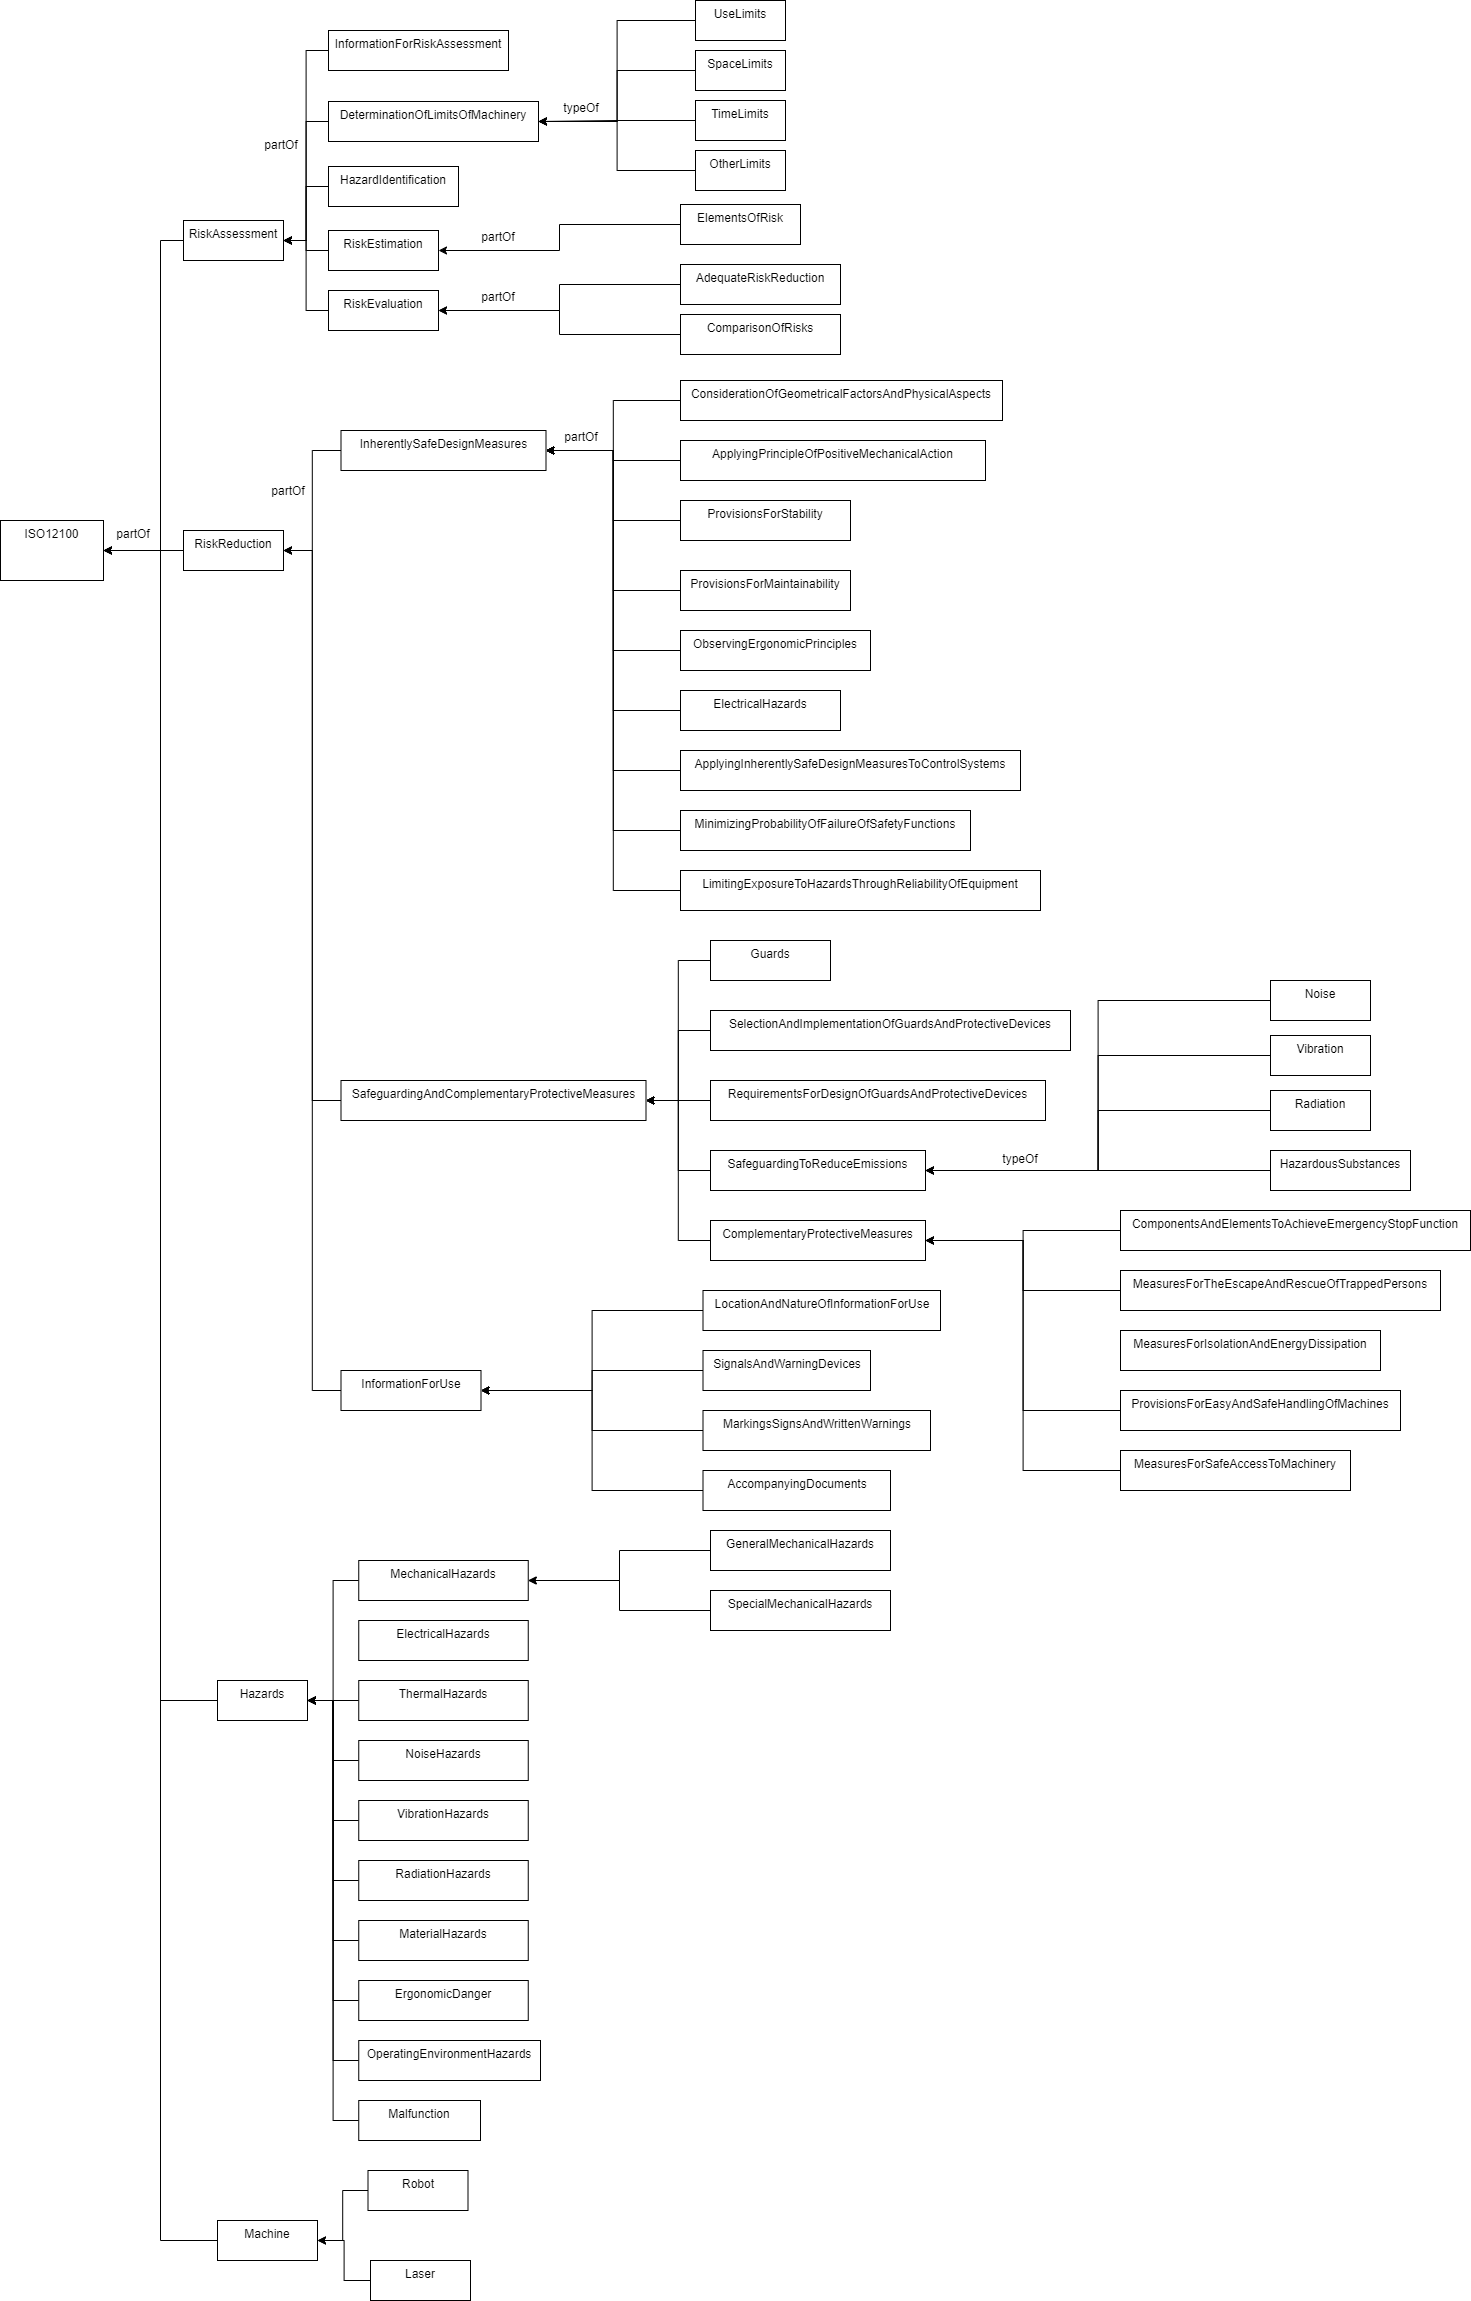
\includegraphics[width=\textwidth]{img/Class_Hierarchy.png}

\paragraph{} For this thesis, the model defined starts with a broad concept "ISO12100". However, it is possible to go on higher level than this if more safety standards are to be added to the model. For example, with the concept "Safety\_Standards" as a level before and child concepts like "Type\_A\_Standards", "Type\_B\_Standards", "Type\_C\_Standards" and then under "Type\_A\_Standards" would come "ISO12100". This could be useful if a knowledge model for other safety standards are also created for different types of standards.

%\bigskip
%\begin{center}
%   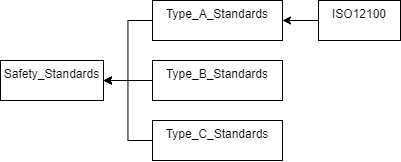
\includegraphics[scale=0.5]{img/Model_Extent.png}
%    %\caption{Possibility of extension on a higher level}
%\end{center}

\bigskip \adjustimage{scale=0.5, center, caption={Possibility of extension on a higher level}, label={fig5}, nofloat=figure, vspace=\bigskipamount}{img/Model_Extent.png}

\paragraph{} To understand the depth of the model, one Instance could be taken as an example. ISO12100 has a sub-class RiskReduction which has a sub-class SafeguardingAndComplimentaryProtectiveMeasures which has a subclass ComplimentaryProtectiveMeasures and finally MeasuresForSafeAccessToMachinery.

% \bigskip\bigskip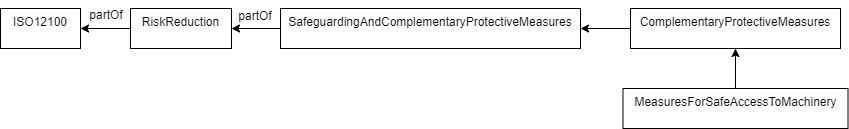
\includegraphics[width=\textwidth]{img/Model_Depth.png}
    %\caption{Depth of the class hierarchy}

\bigskip\bigskip \adjustimage{width=\textwidth, center, caption={Depth of the class hierarchy}, label={fig6}, nofloat=figure, vspace=\bigskipamount}{img/Model_Depth.png}

\adjustimage{width=\textwidth, center, caption={Class hierarchy diagram}, label={fig7}, nofloat=figure, vspace=\bigskipamount}{img/Class_Hierarchy.png}
    
\section{Develop the knowledge model}\label{develop}

Now since the basic outline is drafted, it is required to formalize the information into a knowledge model. OntoBroker \cite{ontobroker} from Semafora Systems is the tool that is used to formalize the SPO triples into a knowledge graph. 

\subsection{Semantic tools used}

\paragraph{OntoBroker: } OntoBroker is the semantic middleware that is used for this project. OntoBroker is a software tool developed by Semafora Systems, which is used for managing and querying ontologies. An ontology is a formal representation of the knowledge in a particular domain, which includes concepts and their relationships, properties and axioms that define these concepts. OntoBroker provides a comprehensive framework for ontology management that includes ontology editing, browsing, querying, and reasoning capabilities. OntoBroker supports multiple ontology languages including OWL, RDF, ObjectLogic. 

\paragraph{ObjectLogic: } ObjectLogic is the primary language for OntoBroker and it is also the language used for this project. ObjectLogic \cite{obl} is a knowledge representation and query language. It explicitly supports data types and have a clean syntax which is easy to understand. In ObjectLogic, knowledge is represented using objects, which have attributes. Objects have relationships to other objects. These objects can be used to model concepts. For the domain of industrial risk assessment, hazards, preventive measures, risks, cause of hazards, etc. are all concepts. ObjectLogic also includes features for defining and reasoning with complex class hierarchies. The complete class sub-class hierarchy is modelled as defined previously in \ref{class_hierarchy}. The main reason of using ObjectLogic is due to its simple syntax which is easy to use even by someone who is not well versed with coding. This makes it easier for the engineers to also contribute and update the knowledge model very easily.

\paragraph{OntoStudio-X: } The development environment used for this project is OntoStudio-X (OSX) \cite{osx}. OntoStudio-X stitches together the advantages of two well-established technical worlds - the tabular format of Microsoft Excel and the inference engine OntoBroker. Through the integration of OntoBroker's function and data structures with Excel's internal object model, it is possible to access all of OntoBroker's functions within the Excel cell structure without the need for Excel VBA. As a result, Excel files containing OntoBroker ontologies and instruction structures can be shared without macros, just like any other .xlsx file. 

% Give screenshots of OSX 3 tabs, 

\subsection{Development of the knowledge graph}

% cite some paper

A knowledge graph is a database that stores and organizes information about concepts or entities (such as people, places, or things) and the relationships between them. Unlike traditional databases that store data in tables, knowledge graphs represent data as nodes and edges in a graph structure. Each node represents an entity and each edge represents a relationship between two entities. General information about a knowledge graph can be cited from the work of Hogan et al. \cite{Hogan_2021}. For example, a knowledge graph might represent a machine as a node and the hazard linked to it as an edge connecting it to another node representing the hazard name which can further be expanded to have information about the preventive measures against the hazard, location of the hazard and so on that can actually help in speeding up the risk assessment process. This makes a knowledge graph to be a perfect candidate to be used for this project. Also the data collected is in SPO format makes the work much simpler to achieve a knowledge graph pertaining to their similar structure. Hence, Hypothesis 2 proposed can be considered to be effective.

\paragraph{} Until this point, the unstructured data from the safety standard and expert's documented knowledge is already collected in a structured format as SPO (Subject-Predicate-Object) triples. Now it is required to formalize this data according to ObjectLogic's syntax to develop the final knowledge graph. An automatic approach is preferred to do so using a Python script. It is beneficial to follow this approach for the following reasons:
\begin{enumerate}
    \item \textbf{Consistency: }A Python script can be used to formalize SPO triples into a knowledge graph with a consistent structure, ensuring that all the data is organized and stored in a standardized manner. This makes it easier to analyze and extract insights when querying the data. For this project, the camel case naming convention is used in general. The upper camel case is considered for the concepts (- subjects and objects) and the lower camel case for the relations.
    % Example flowchart visual
    \item \textbf{Automation: }Using a Python script to formalize SPO triples into a knowledge graph can automate the process, which saves time and reduces the risk of errors that can occur when manually entering data into a graph.
    \item \textbf{Flexibility: }Python is a versatile language that offers a wide range of tools and libraries for data processing and analysis. This makes it easily possible to customize the script to suit specific requirements, such as filtering or transforming the data before or even after it is added to the knowledge graph. Even while building the knowledge model at times it was required to change the format of few data. These changes were done very easily by the code that is used to transform the SPO triples to knowledge graph.
    \item \textbf{Scalability: }Formalizing SPO triples into a knowledge graph using a Python script can be scaled up to handle large volumes of data. This makes it really easy for future expansion of the knowledge graph with several other safety standards.
\end{enumerate}

The column containing the SPO triples from the excel sheet is taken as input. The triples are already structured in a dictionary with the subject object and relation tagged separately. The list of dictionary is looped through to work on each content of the list. First the naming convention is taken care of. Each phrase is split for words and then the first letter of each word is capitalized. Then all the letters are joined together into a single string. For the function of upper camel case, which is used for the subjects and objects, all the initial letters of each word are capitalized and for the function of lower camel case, which is used for the relations, all the initial letters of each word are capitalized except the first word. After naming, the concepts and relations are structured into the schema defination of ObjectLogic as defined in \cite{obl}. The list of formatted output is taken into a pandas dataframe so that it is easier to write on the Excel interface of the OntoStudio-X. A screenshot of the schema in OntoStudio-X is shown below:

% \bigskip\bigskip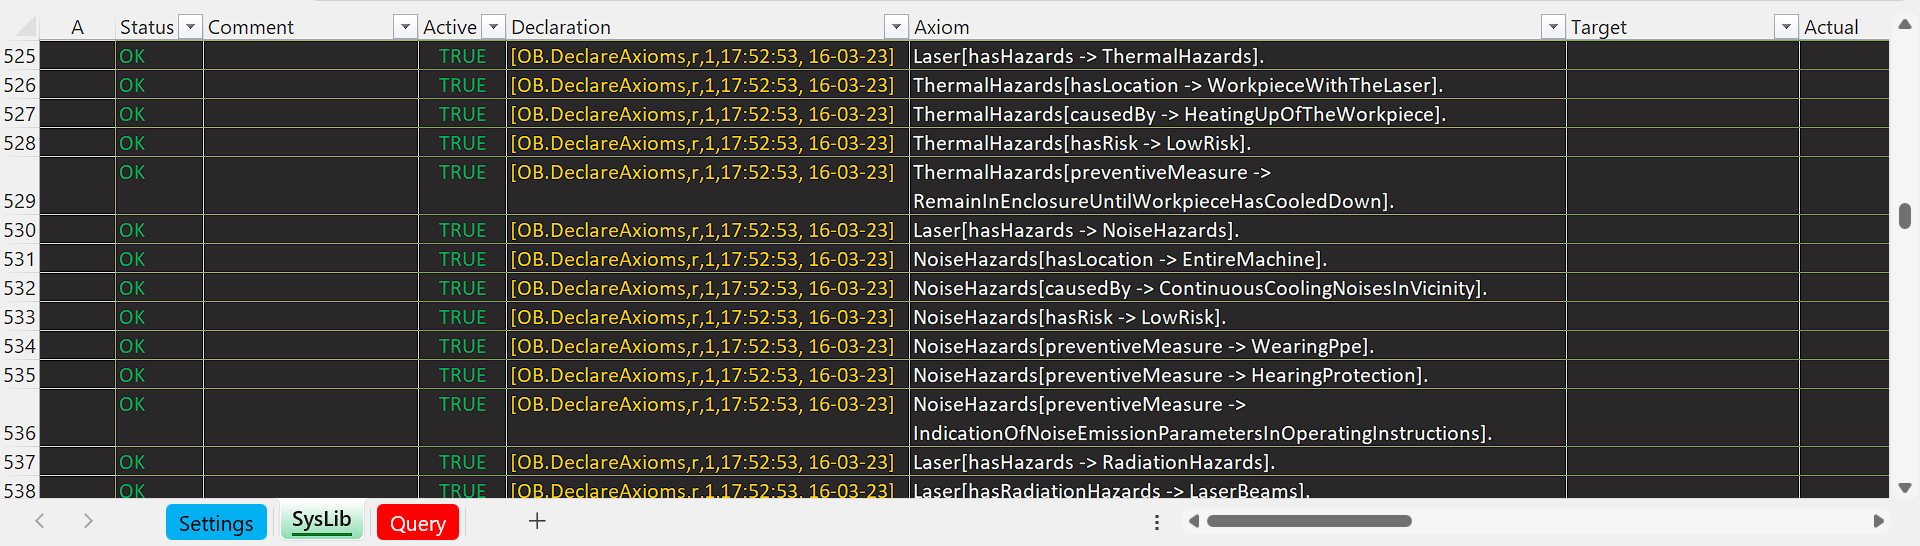
\includegraphics[width=\textwidth, height=150pt] {img/OSX_Schema.png}

\bigskip\bigskip \adjustimage{width=\textwidth, height=150pt, center, caption={Concepts and relations schema in OntoStudio-X}, label={fig8}, nofloat=figure, vspace=\bigskipamount}{img/OSX_Schema.png}

\paragraph{}Even before formalizing the concepts and relation into OntoBroker, the class and subclass must be defined, according to \cite{Luo2016}. Similar approach as before is taken in doing so. The class names are structured in upper camel case and the schema is defined according to the syntax in \cite{obl}. The list of class and subclass structure is then written to the Excel interface of the OntoStudio-X. An example screenshot of the class structure in OntoStudio-X is shown below:

% \bigskip\bigskip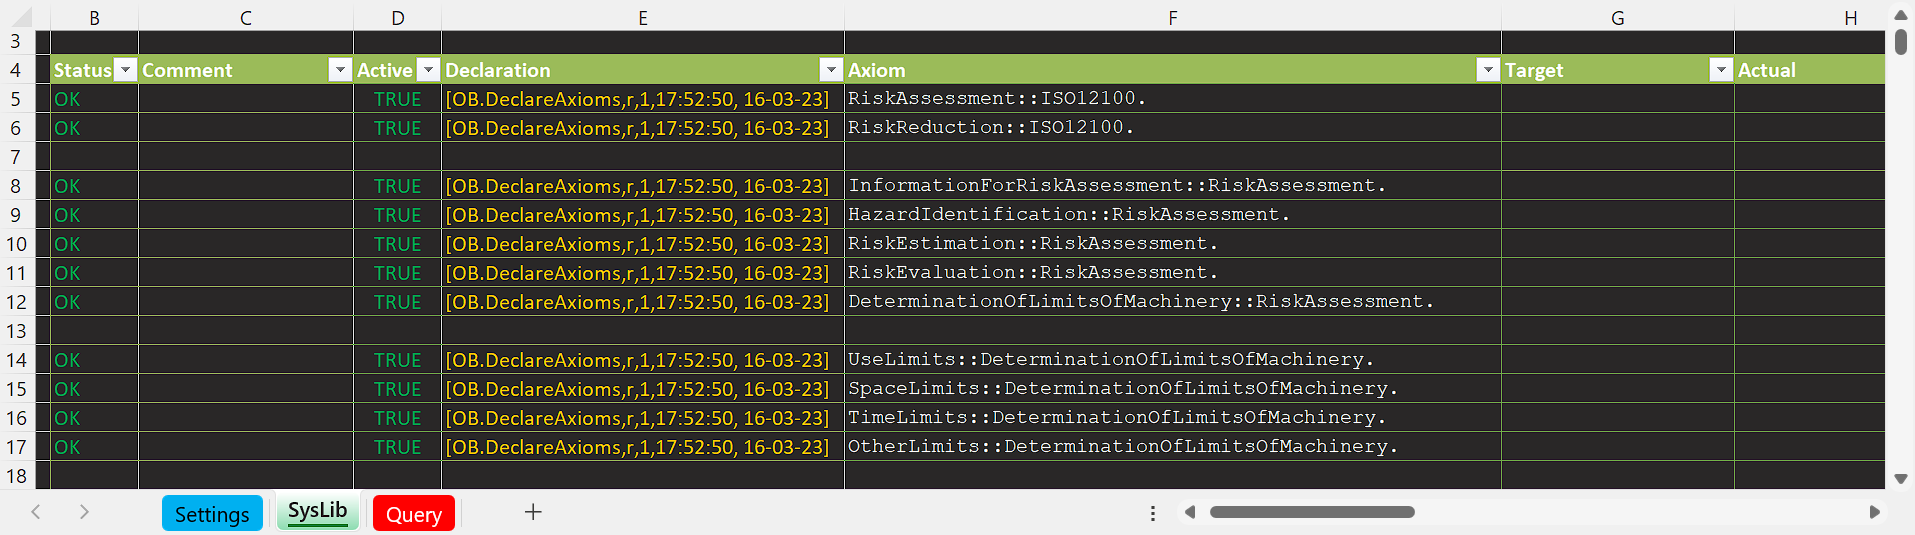
\includegraphics[width=\textwidth, height=150pt]{img/OSX_Class.png}

\bigskip\bigskip \adjustimage{width=\textwidth, height=150pt, center, caption={Class sub-class structure in OntoStudio-X}, label={fig9}, nofloat=figure, vspace=\bigskipamount}{img/OSX_Class.png}